%! suppress = UnresolvedReference


\chapter{\app 的设计}\label{ch:design}


\section{项目的整体架构设计}\label{sec:arch-design}

\subsection{Git子模块介绍}\label{subsec:git-submodule}

Git子模块(submodule)允许将一个Git仓库作为另一个Git仓库的子目录。为了方便项目管理,本项目的内容被拆分到了多个Git仓库,各个仓库之间的一些共享的部分使用了Git子模块来实现复用与同步。

与Git子模块功能类似的工具还有Git子树(subtree)等,但其他工具对于在主仓库修改之后向子仓库进行推送的这一需求都没有像Git子模块这样的良好支持,再考虑到整个项目架构的一致性,本项目在内部各个仓库之间的依赖方式上都选择了Git子模块作为解决方案(对外部仓库的依赖方式则有所不同)。

\subsection{项目包含的Git仓库}\label{subsec:git-repositories}

本项目在整体架构上一共由7个Git仓库组成,这些仓库的名称以及仓库之间的子模块关系如图~\ref{fig:repositories}所示。

\begin{figure}[h]
    \centering
    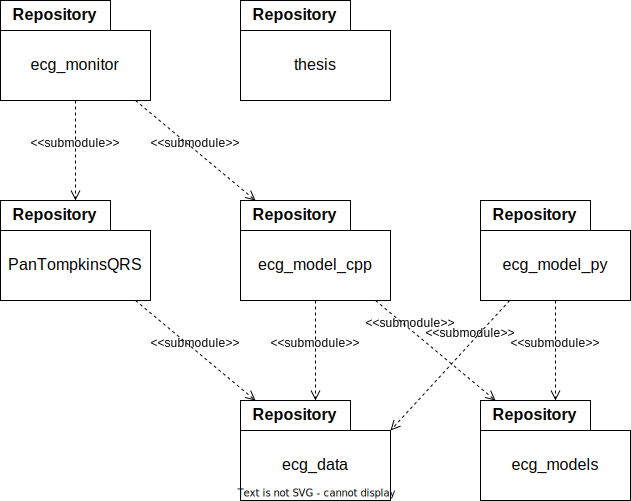
\includegraphics[width=\textwidth]{../assets/repositories.drawio}
    \bicaption{项目包含的Git仓库}{Git repositories of the project}
    \label{fig:repositories}
\end{figure}

\subsubsection{thesis}\label{subsubsec:repo-thesis}

这是本篇论文所在的仓库。论文本身作为项目文档的一部分,也被包含在本项目之中。该仓库包含论文的\LaTeX 源码,以及论文中引用的图片等资源文件,还有自动格式化、依赖版本管理、自动构建测试、自动发布新版本等持续集成配置。

论文与应用本身的代码是分离的,所以论文的仓库与应用的仓库之间没有任何子模块关系。此外,论文仓库以Git子树的形式包含了论文模板\footnote{\url{https://github.com/Koyamin/ECNUThesis-Undergraduate}},没有使用Git子模块是因为基于模板进行编写后只需要直接提交至主仓库,不需要向子仓库推送,这与~\ref{subsec:git-submodule} 节所述的情况不同。

\subsubsection{ecg\_monitor}\label{subsubsec:repo-monitor}

这是应用的主体仓库。该仓库包含基于Flutter框架编写的Dart代码,以及相关的各种配置文件等。仓库的命名与应用的包名一致,因此按照Dart对包名的相关限制使用了小写下划线的命名风格,而非Git仓库常用的小写连字符。为了保持项目各个仓库之间的一致性,其他仓库(除PanTompkinsQRS外)也都使用了小写下划线的命名风格。

为了方便调用C++代码,该仓库以Git子模块的形式包含了PanTompkinsQRS和ecg\_model\_cpp两个子仓库,这两个子仓库分别提供了Pan-Tompkins算法和基于LibTorch的心电图智能分析算法的实现。

\subsubsection{PanTompkinsQRS}\label{subsubsec:repo-qrs}

这是应用中用于实现Pan-Tompkins算法的仓库。该仓库是rafaelmmoreira编写的Pan-Tompkins算法的C语言实现\footnote{\url{https://github.com/rafaelmmoreira/PanTompkinsQRS}}的复刻(fork),在原始版本的基础上根据项目需要进行了一些修改。出于对原作者的尊重,该仓库的名称与原作者的命名保持一致,因此与项目内其他仓库的命名风格不同。

该仓库被ecg\_monitor所包含,并且为了方便测试而将ecg\_data包含为了子仓库,后者提供了一些测试用的心电图数据,用作测试时的输入。

\subsubsection{ecg\_model\_cpp}\label{subsubsec:repo-cpp}

这是应用中用于实现基于LibTorch的心电图智能分析算法的仓库。该仓库是ecg\_model\_py仓库的C++实现,使用了LibTorch作为框架。

该仓库被ecg\_monitor所包含,且包含了ecg\_data作为测试输入数据,还包含了ecg\_models作为与ecg\_model\_py共享的模型文件以及测试预期输出。

\subsubsection{ecg\_model\_py}\label{subsubsec:repo-py}

这是基于PyTorch实现的心电图智能分析算法的所在仓库。该仓库以算法的原始版本作为初始提交,在此基础上根据项目需要进行了修改。

Python版本的算法并不直接被应用调用,因此该仓库不是其他仓库的子模块。该仓库包含了ecg\_data作为测试输入数据,将与ecg\_model\_cpp共享的模型文件保存在ecg\_models,并将PyTorch版本的算法输出也写入ecg\_models子模块以便与ecg\_model\_cpp共享。

\subsubsection{ecg\_data}\label{subsubsec:repo-data}

该仓库存储了各算法仓库用作测试输入的心电图数据,以及从公开数据库下载心电数据并转换格式的相关代码。该仓库中的数据由仓库内的代码写入,被上述三个算法仓库所读取。

\subsubsection{ecg\_models}\label{subsubsec:repo-models}

该仓库存储了TorchScript模型文件,以及模型在测试输入下的输出结果。该仓库的内容由ecg\_model\_py写入,被ecg\_model\_cpp读取。因为模型文件较大(60多MB),且不被Pan-Tompkins算法所需要,所以该仓库与ecg\_data进行了分离。


\section{应用的界面与功能设计}\label{sec:app-design}

\subsection{应用的界面设计规范}\label{subsec:app-design-spec}

本应用与其他同类应用的一大差别在于其遵循专业的设计规范对应用界面进行了严格的设计。

应用整体上遵循Material 3设计规范\cite{MaterialDesign}。Material 3(也称为Material You)是Google在2021年5月的Google I/O大会上宣布的新一代Material设计规范,和前代规范相比具有从用户的壁纸自动生成动态主题颜色、按钮更大、界面动画更多等新特性,并在其他一些细节设计上有所优化。目前Material 3设计已被广泛应用于Google的各种应用程序,并成为Android应用的推荐设计规范。

尽管Material 3按照Google的设计是可以在任何平台(包括iOS)上使用的,但从事实上来说,iOS应用确实较少使用Material风格的设计,而较多按照苹果的推荐遵循Cupertino\footnote{苹果官方并未给自己的设计规范进行像Material这样的明确命名,Cupertino这个名字是Flutter在其文档中使用的,可能是基于苹果总部位于美国加利福尼亚州丘珀蒂诺(Cupertino)市的事实。}设计。为了符合iOS平台的用户习惯,本应用在iOS平台上将部分UI组件替换为了iOS应用常用的Cupertino风格的组件。由于Cupertino并未像Material一样提供全平台可用的设计,所以应用的设计仍然以Material为主,在Android平台上完全使用Material 3风格的设计,而在iOS平台上则使用Material 3风格与Cupertino风格的混合设计,如图~\ref{fig:android-ios} 所示。

\begin{figure}[h]
    \subcaptionbox{Android}{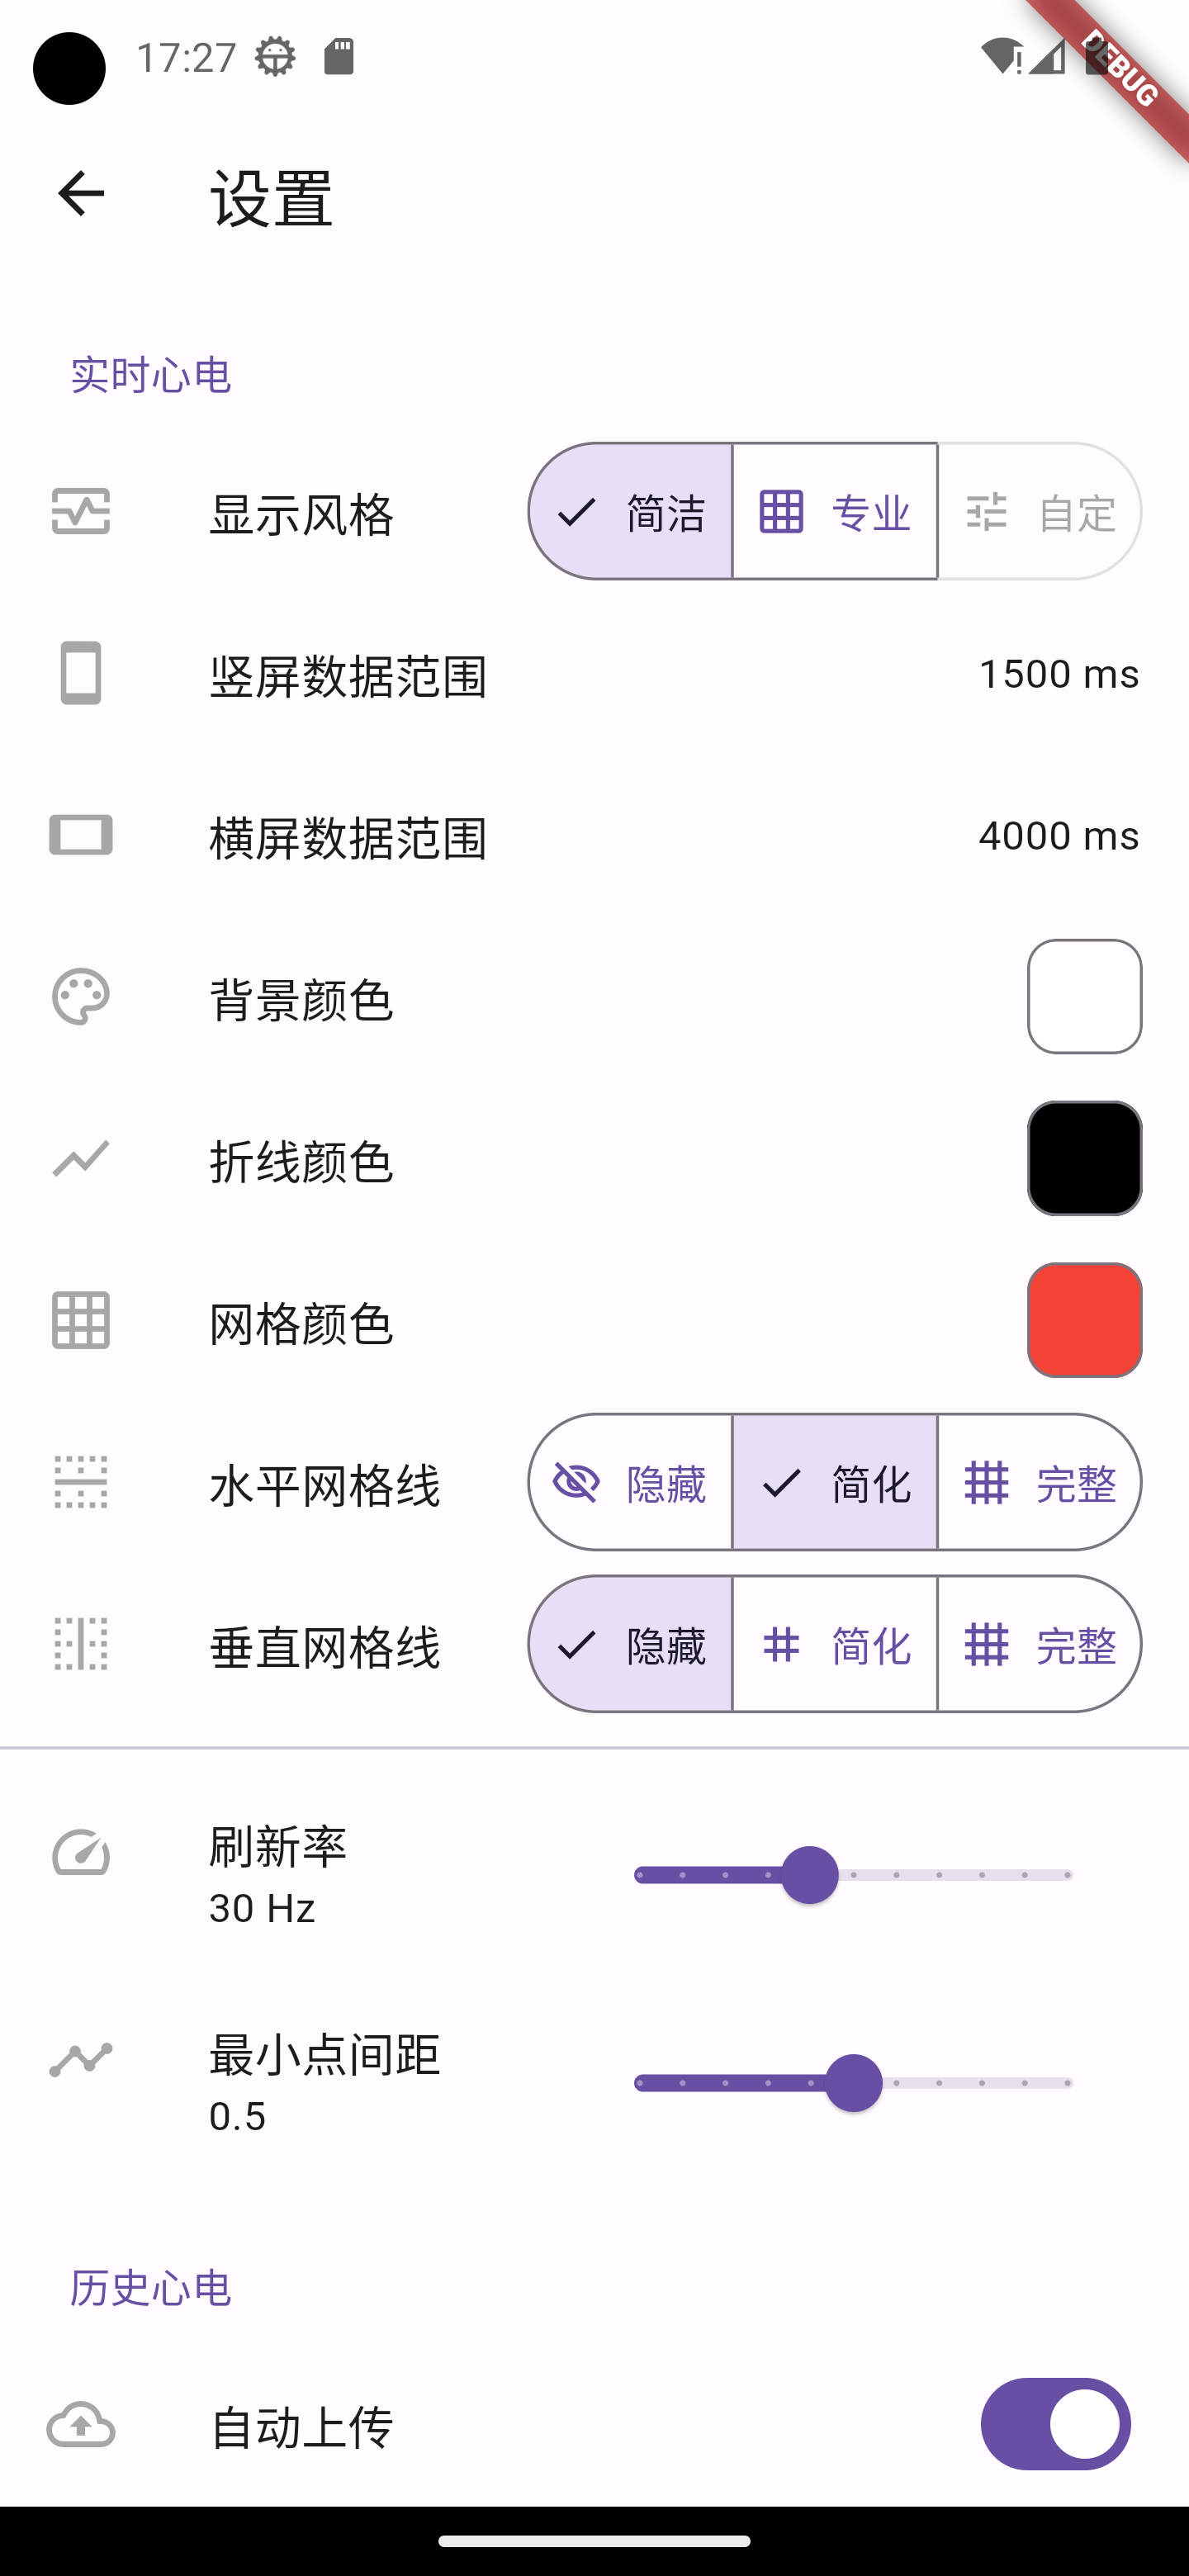
\includegraphics[height=17cm]{../assets/settings}}
    \subcaptionbox{iOS}{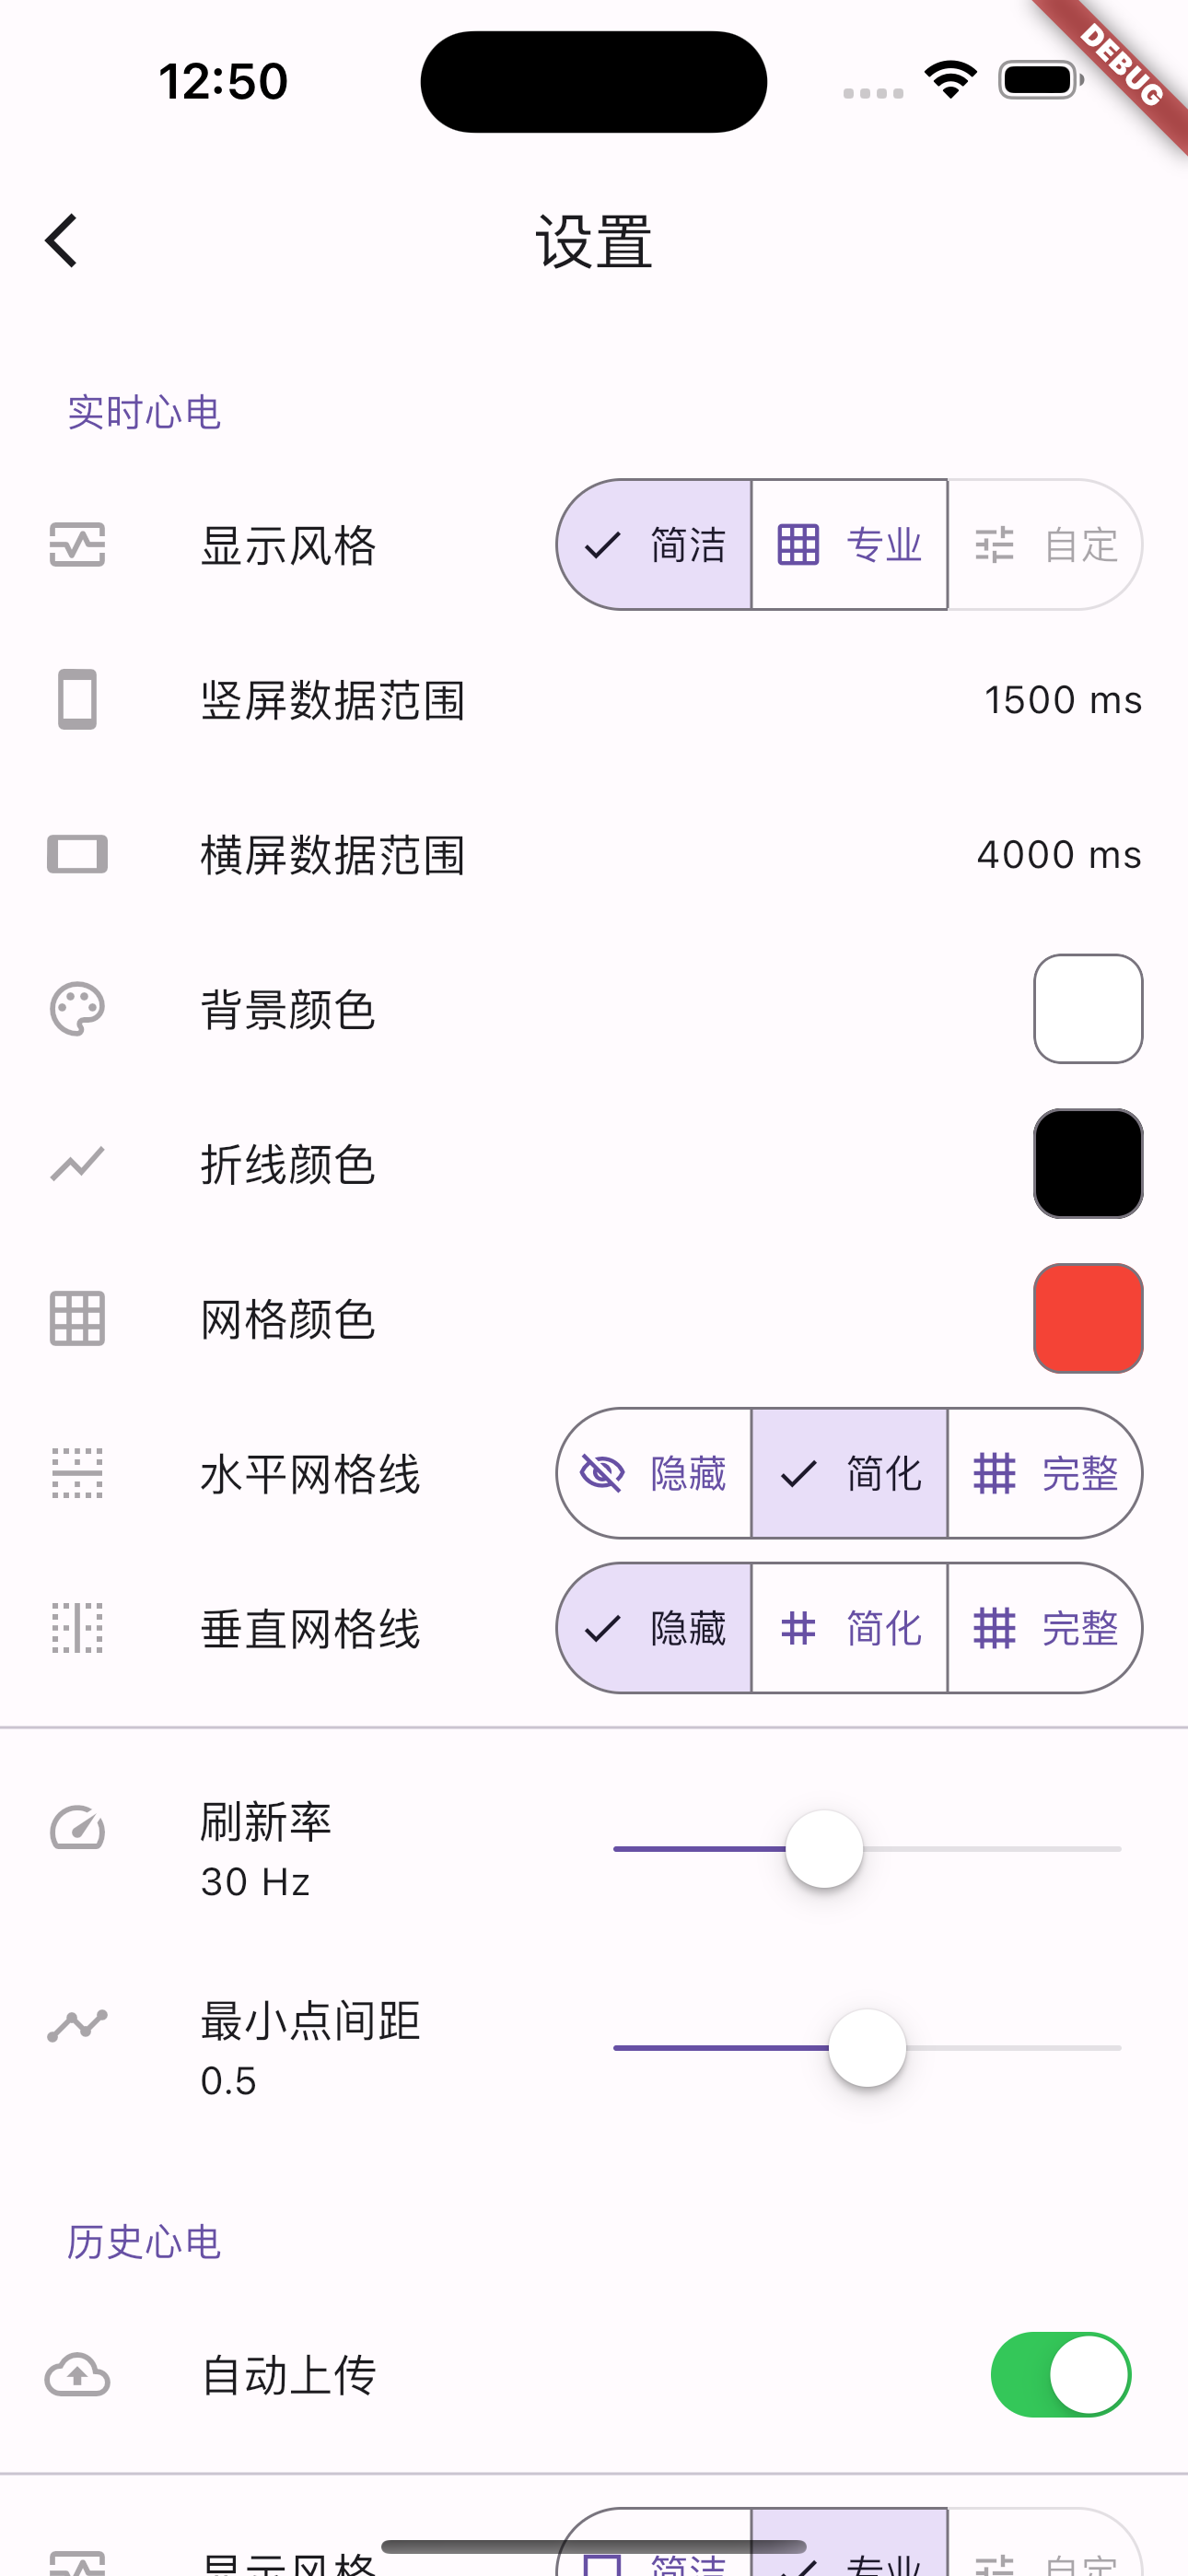
\includegraphics[height=17cm]{../assets/ios-settings}}
    \bicaption{应用在Android和iOS平台上的界面设计对比}{Comparison of the app's UI design on Android and iOS}
    \label{fig:android-ios}
\end{figure}

从图~\ref{fig:android-ios} 中可以看出应用在Android平台与iOS平台上的界面设计的一些差异,包括标题的对齐方式(Android居左,iOS居中)、左上角返回按钮的图标(Android使用完整箭头,iOS使用仅有头部的简化箭头)、滑动条与切换按钮的外观(按照各自规范中的相关要求)、文本的字体(iOS的字体更细)等。

\subsection{实时心电页面的设计}\label{subsec:real-time-design}

\subsubsection{心电图纸}\label{subsubsec:ecg-paper}

% 心电图纸包含红色的坐标线,每1mm一小格(用细线分隔),每5mm一大格(用粗线分隔)。横轴一小格表示40ms,一大格表示200ms。纵轴一小格表示0.1mV,一大格表示0.5mV。

\todo{实时心电页面的设计}

\subsection{历史心电页面的设计}\label{subsec:history-design}

\todo{历史心电页面的设计}

\subsection{分析报告页面的设计}\label{subsec:analytics-design}

\todo{分析报告页面的设计}

\subsection{设备管理页面的设计}\label{subsec:device-design}

\todo{设备管理页面的设计}

\subsection{我的页面的设计}\label{subsec:me-design}

\todo{我的页面的设计}

\subsection{应用设置页面的设计}\label{subsec:settings-design}

\todo{应用设置页面的设计}


\section{应用的数据库设计}\label{sec:db-design}

\todo{数据库设计}
